\documentclass[10pt]{article}
\usepackage[a4paper,margin=18mm]{geometry}
\usepackage[T1]{fontenc}\usepackage{lmodern}
\usepackage{amsmath,amssymb,booktabs,array,enumitem}
\usepackage{tikz}\usetikzlibrary{shapes.gates.logic.US,positioning,arrows.meta}
\usepackage[hidelinks]{hyperref}
\setlength{\parindent}{0pt}\setlength{\parskip}{4pt}\setlength{\emergencystretch}{2em}
\newcommand{\mos}[4]{\begin{scope}[shift={(#1,#2)}]
\draw(0,.24)--(0,-.24);\draw(0,.2)--(.25,.2)--(.25,.5);\draw(0,-.2)--(.25,-.2)--(.25,-.5);
\draw(-.16,.23)--(-.16,-.23);
\ifnum#4=1\draw(-.26,0)circle(.06);\draw(-.75,0)--(-.32,0);\else\draw(-.75,0)--(-.16,0);\fi
\node[anchor=east,font=\scriptsize]at(-.76,0){$#3$};\end{scope}}
\newcommand{\gnd}[2]{\draw(#1,#2)--(#1,{#2-.12});\draw({#1-.17},{#2-.12})--({#1+.17},{#2-.12});\draw({#1-.11},{#2-.2})--({#1+.11},{#2-.2});}
\newcommand{\rail}[3]{\draw(#1,#2)--(#1,{#2+.14});\node[above,font=\scriptsize]at(#1,{#2+.14}){$#3$};}
\begin{document}
\begin{center}\large\textbf{2023 Midterm -- Corrected Solutions}\\\normalsize Complete source questions 5--7 only\end{center}
\textbf{Scope and method.} The original photograph supplies Q5--7 (35 points) and a fragment of Q4. Q4 is not solved because its threshold/resistance premise is missing. Student answers were compared after deriving the surviving questions; grades establish provenance, not correctness. All diagrams below are editable TikZ. Checks are analytical, with no process simulation.

\section*{Question 5: noise margins and sensitization}
Let $q=G1=\overline{BC}$, $G2=\overline{A+q}$ and $G3=\overline{qD}$. A single $W/L$ nMOS and a $2W/L$ pMOS have equal strength because $\mu_n=2\mu_p$:
\[\beta_n=\mu_nC_{ox}W/L=\mu_pC_{ox}(2W/L)=\beta_p=\beta.\]
For a sensitized NAND input, the nMOS series network is weaker than the pMOS pull-up; the usual equivalent strengths are $\beta_n/2$ and $\beta_p$. For a sensitized NOR input, the pMOS series network is weaker; the equivalent strengths are $\beta_p/2$ and $\beta_n$.

\textbf{Conventional qualitative answer.} Under the standard matched-threshold static-CMOS voltage-transfer model with ideal output rails,
\[\boxed{G1:\ NM_L>NM_H,\qquad G2:\ NM_L<NM_H,\qquad G3:\ NM_L>NM_H.}\]
A stronger p-network shifts the transfer characteristic toward larger input voltages, favoring $NM_L$; a stronger n-network shifts it the other way. The paper supplies no threshold magnitudes or $V_{DD}$ for this question. Consequently it determines no numerical margins; the comparison above is explicitly conditional on conventional VTC symmetry.

\begin{center}\begin{tabular}{ccccp{7.2cm}}\toprule
$ABCD$&$q$&$G2$&$G3$&Single-input context\\\midrule
0011&1&0&0&$A=0$ sensitizes the $q$ input of G2; $D=1$ sensitizes the $q$ input of G3.\\
0101&1&0&0&Same downstream sensitization; the zero input of G1 is now $C$.\\
1101&1&0&0&G2 has both inputs high. Either other fixed-high input masks a disturbance on only one input.\\
1110&0&0&1&G2 is sensitized to $A$ because $q=0$; G3 has both inputs low, so either other fixed-low input masks a disturbance on only one input.\\\bottomrule
\end{tabular}\end{center}

For the two masked contexts, there is no switching transfer curve for just the disturbed input with the other input fixed at that rail. This does not contradict the structural NAND/NOR margin comparison. Simultaneous input noise is a different experiment; in the simple parallel/series-strength approximation its ratios are $\beta_p/\beta_n=1/4$ for the tied-input NOR and $4$ for the tied-input NAND, preserving the same qualitative bias.

Both student sets identify the same conventional inequalities. The final answer adds the missing model qualification and distinguishes the source patterns, including $1110$ exactly as printed. No student-derived threshold values are inserted into this question.

\newpage\section*{Question 6: a six-transistor AND with $7RC_g$ delay}
Use a two-input NAND followed by an inverter. Choose each NAND nMOS and pMOS $2W/L$; choose the inverter nMOS $W/L$ and pMOS $2W/L$. Tie every pMOS body to $V_{DD}$ and every nMOS body to ground.
\begin{center}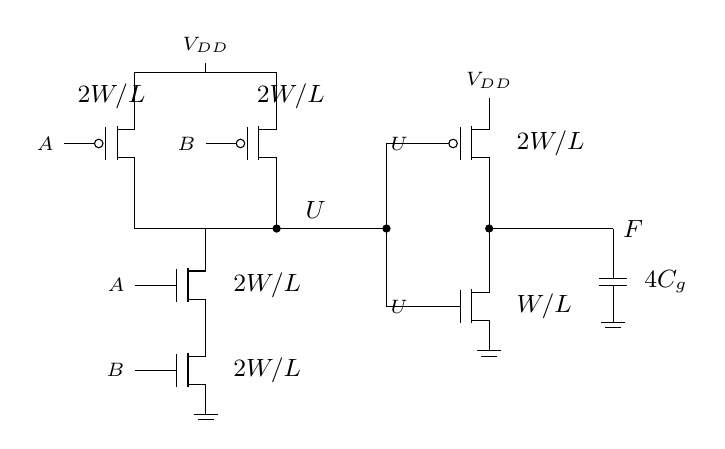
\begin{tikzpicture}[x=.9cm,y=.9cm,font=\small]
\mos{0}{3}{A}{1}\mos{2}{3}{B}{1}
\draw(.25,3.5)--(.25,4)--(2.25,4)--(2.25,3.5);\rail{1.25}{4}{V_{DD}};
\draw(.25,2.5)--(.25,1.8)--(2.25,1.8)--(2.25,2.5);\draw(1.25,1.8)--(1.25,1.5);
\mos{1}{1}{A}{0}\mos{1}{-.2}{B}{0}\draw(1.25,.5)--(1.25,.3);\gnd{1.25}{-.7}
\node at(-.08,3.66){$2W/L$};\node at(2.45,3.66){$2W/L$};\node[right]at(1.5,1){$2W/L$};\node[right]at(1.5,-.2){$2W/L$};
\draw(2.25,1.8)--(3.5,1.8);\node[above]at(2.8,1.8){$U$};\fill(2.25,1.8)circle(1.5pt);
\mos{5}{3}{U}{1}\mos{5}{.7}{U}{0}\rail{5.25}{3.5}{V_{DD}};\gnd{5.25}{.2};\draw(5.25,2.5)--(5.25,1.2);
\draw(3.5,1.8)--(3.8,1.8)--(3.8,3)--(4.25,3);\draw(3.8,1.8)--(3.8,.7)--(4.25,.7);\fill(3.8,1.8)circle(1.5pt);
\node[right]at(5.5,3){$2W/L$};\node[right]at(5.5,.7){$W/L$};
\draw(5.25,1.8)--(7,1.8)node[right]{$F$};\fill(5.25,1.8)circle(1.5pt);\draw(7,1.8)--(7,1.1);\draw(6.8,1.1)--(7.2,1.1);\draw(6.8,1)--(7.2,1);\draw(7,1)--(7,.6);\gnd{7}{.6};\node[right]at(7.3,1.05){$4C_g$};
\end{tikzpicture}\end{center}
Here $C_g$ is the capacitance of \emph{one} $W/L$ transistor. The inverter loads the NAND with $(1+2)C_g=3C_g$. A NAND nMOS has resistance $R/2$, so two in series have $R$. Each NAND pMOS has $R$ because its mobility is half and width twice the nMOS reference; the worst pull-up uses one pMOS. Both inverter resistances are $R$.
\begin{center}\begin{tabular}{lccc}\toprule
AND transition&NAND delay&Inverter delay&Total\\\midrule
Output rise&$R(3C_g)$&$R(4C_g)$&$7RC_g$\\
Output fall&$R(3C_g)$&$R(4C_g)$&$7RC_g$\\\bottomrule
\end{tabular}\end{center}
Thus $\boxed{t_{worst}=7RC_g<8RC_g}$. This uses the stipulated RC-sum model, neglects parasitics as directed, and is not a process-dependent measured delay. Student set A already gives a compatible sizing and $3C_g$ internal load; it is retained with a complete transistor/capacitance accounting. The independent checker verifies all four logic states and both transition paths.

\newpage\section*{Question 7(a): $F=X(Y+Z)+XW$}
Factor the original positive-polarity function:
\[F=X(Y+Z+W).\]
Build an inverting complex gate with internal output $U=\overline{X(Y+Z+W)}$, then a static inverter $F=\overline U$. The core nMOS network is $X$ in series with parallel $Y,Z,W$; its dual pMOS network is $X$ in parallel with series $Y,Z,W$.
\begin{center}\begin{tikzpicture}[x=.75cm,y=.75cm,font=\small]
\mos{0}{2.55}{X}{1}
\draw(.25,3.05)--(.25,4.3)--(3.25,4.3);\rail{1.6}{4.3}{V_{DD}};\draw(.25,2.05)--(.25,.25);
\mos{3}{3.45}{Y}{1}
\mos{3}{2.35}{Z}{1}
\mos{3}{1.25}{W}{1}
\draw(3.25,4.3)--(3.25,3.95);
\draw(3.25,2.95)--(3.25,2.85);
\draw(3.25,1.85)--(3.25,1.75);
\draw(3.25,0.75)--(3.25,.25);
\mos{0}{-.75}{X}{0}
\draw(.25,.25)--(.25,-.25);\draw(.25,-1.25)--(.25,-1.55);
\draw(.25,-1.55)--(4.25,-1.55);\draw(.25,-3.05)--(4.25,-3.05);
\mos{0}{-2.3}{Y}{0}\draw(0.25,-1.55)--(0.25,-1.8);\draw(0.25,-2.8)--(0.25,-3.05);
\mos{2}{-2.3}{Z}{0}\draw(2.25,-1.55)--(2.25,-1.8);\draw(2.25,-2.8)--(2.25,-3.05);
\mos{4}{-2.3}{W}{0}\draw(4.25,-1.55)--(4.25,-1.8);\draw(4.25,-2.8)--(4.25,-3.05);
\gnd{1.3}{-3.05};
\draw(.25,.25)--(4.85,.25);\fill(3.25,.25)circle(1.5pt);\node[above]at(4.35,.25){$U$};
\mos{7}{2}{U}{1}\mos{7}{-1}{U}{0}
\rail{7.25}{2.5}{V_{DD}};\gnd{7.25}{-1.5};\draw(7.25,1.5)--(7.25,-.5);
\draw(4.85,.25)--(5.7,.25)--(5.7,2)--(6.25,2);\draw(5.7,.25)--(5.7,-1)--(6.25,-1);\fill(5.7,.25)circle(1.5pt);
\draw(7.25,.25)--(8.2,.25)node[right]{$F$};\fill(7.25,.25)circle(1.5pt);
\end{tikzpicture}\end{center}
The eight-transistor core plus the two-transistor output inverter uses 10 transistors. For $X=0$ the pMOS $X$ holds $U=1$ and $F=0$. For $X=1$, any of $Y,Z,W=1$ completes a pull-down path at $U$, giving $F=1$; otherwise the series pMOS path holds $U=1$. All pMOS bodies connect to $V_{DD}$; all nMOS bodies connect to ground. Gate labels on the inverter are $U$, not new primary inputs.

Both student sets use a De Morgan construction involving complemented primary inputs. That approach can be valid if the complements are generated, but the visible drawings do not supply their input inverters. The factored implementation above needs only original inputs and preserves the positive output polarity without assuming free complements.

\newpage\section*{Question 7(b): $F=\overline{X(Y+Z)}$}
This output is already inverting. Use a six-transistor core directly: nMOS $X$ in series with parallel $Y,Z$, pMOS $X$ in parallel with series $Y,Z$.
\begin{center}\begin{tikzpicture}[x=.75cm,y=.75cm,font=\small]
\mos{0}{2.55}{X}{1}
\draw(.25,3.05)--(.25,4.3)--(3.25,4.3);\rail{1.6}{4.3}{V_{DD}};\draw(.25,2.05)--(.25,.25);
\mos{3}{3.45}{Y}{1}
\mos{3}{2.35}{Z}{1}
\draw(3.25,4.3)--(3.25,3.95);
\draw(3.25,2.95)--(3.25,2.85);
\draw(3.25,1.85)--(3.25,.25);
\mos{0}{-.75}{X}{0}
\draw(.25,.25)--(.25,-.25);\draw(.25,-1.25)--(.25,-1.55);
\draw(.25,-1.55)--(2.25,-1.55);\draw(.25,-3.05)--(2.25,-3.05);
\mos{0}{-2.3}{Y}{0}\draw(0.25,-1.55)--(0.25,-1.8);\draw(0.25,-2.8)--(0.25,-3.05);
\mos{2}{-2.3}{Z}{0}\draw(2.25,-1.55)--(2.25,-1.8);\draw(2.25,-2.8)--(2.25,-3.05);
\gnd{1.3}{-3.05};
\draw(.25,.25)--(4.85,.25);\fill(3.25,.25)circle(1.5pt);\node[above]at(4.35,.25){$F$};
\end{tikzpicture}\end{center}
The PDN conducts exactly when $X(Y+Z)=1$; the dual PUN conducts exactly when $X=0$ or both $Y=Z=0$. Thus $F=\overline{X(Y+Z)}$ for every input, with no output inverter. Both student sets' visible Q7(b) networks agree with this topology. In particular, the two right-side pMOS devices are in series; drawing them in parallel would change the function. Body ties follow the convention above.

\newpage\section*{Question 7(c): $F=XY+YZ$}
Factor $F=Y(X+Z)$. Form $U=\overline{Y(X+Z)}$ with nMOS $Y$ in series with parallel $X,Z$ and the dual pMOS $Y$ in parallel with series $X,Z$. Add a static inverter to restore the positive function.
\begin{center}\begin{tikzpicture}[x=.75cm,y=.75cm,font=\small]
\mos{0}{2.55}{Y}{1}
\draw(.25,3.05)--(.25,4.3)--(3.25,4.3);\rail{1.6}{4.3}{V_{DD}};\draw(.25,2.05)--(.25,.25);
\mos{3}{3.45}{X}{1}
\mos{3}{2.35}{Z}{1}
\draw(3.25,4.3)--(3.25,3.95);
\draw(3.25,2.95)--(3.25,2.85);
\draw(3.25,1.85)--(3.25,.25);
\mos{0}{-.75}{Y}{0}
\draw(.25,.25)--(.25,-.25);\draw(.25,-1.25)--(.25,-1.55);
\draw(.25,-1.55)--(2.25,-1.55);\draw(.25,-3.05)--(2.25,-3.05);
\mos{0}{-2.3}{X}{0}\draw(0.25,-1.55)--(0.25,-1.8);\draw(0.25,-2.8)--(0.25,-3.05);
\mos{2}{-2.3}{Z}{0}\draw(2.25,-1.55)--(2.25,-1.8);\draw(2.25,-2.8)--(2.25,-3.05);
\gnd{1.3}{-3.05};
\draw(.25,.25)--(4.85,.25);\fill(3.25,.25)circle(1.5pt);\node[above]at(4.35,.25){$U$};
\mos{7}{2}{U}{1}\mos{7}{-1}{U}{0}
\rail{7.25}{2.5}{V_{DD}};\gnd{7.25}{-1.5};\draw(7.25,1.5)--(7.25,-.5);
\draw(4.85,.25)--(5.7,.25)--(5.7,2)--(6.25,2);\draw(5.7,.25)--(5.7,-1)--(6.25,-1);\fill(5.7,.25)circle(1.5pt);
\draw(7.25,.25)--(8.2,.25)node[right]{$F$};\fill(7.25,.25)circle(1.5pt);
\end{tikzpicture}\end{center}
The six-transistor core plus its output inverter uses 8 transistors and needs no complemented primary inputs. If $Y=0$, $U=1$ and $F=0$; if $Y=1$, either $X=1$ or $Z=1$ discharges $U$ and gives $F=1$. As in Q7(a), the students' complemented-input construction requires explicit complement generation to be self-contained.

\section*{Reproduction and coverage}
Run \texttt{python verify.py}. Its saved CSV/JSON results contain four Q5 input contexts, the four Q6 truth states and two RC paths, and all 32 Q7 input combinations. The Q7 verifier independently checks graph reachability, exactly one conducting rail network, and the original Boolean equations. It does not infer missing Q4 parameters or certify unseen earlier questions.
\end{document}
